% Generated by Sphinx.
\def\sphinxdocclass{report}
\documentclass[letterpaper,10pt,english]{sphinxmanual}
\usepackage[utf8]{inputenc}
\DeclareUnicodeCharacter{00A0}{\nobreakspace}
\usepackage{cmap}
\usepackage[T1]{fontenc}
\usepackage{babel}
\usepackage{times}
\usepackage[Bjarne]{fncychap}
\usepackage{longtable}
\usepackage{sphinx}
\usepackage{multirow}


\title{matchApp Documentation}
\date{June 23, 2016}
\release{2}
\author{Grupo10}
\newcommand{\sphinxlogo}{}
\renewcommand{\releasename}{Release}
\makeindex

\makeatletter
\def\PYG@reset{\let\PYG@it=\relax \let\PYG@bf=\relax%
    \let\PYG@ul=\relax \let\PYG@tc=\relax%
    \let\PYG@bc=\relax \let\PYG@ff=\relax}
\def\PYG@tok#1{\csname PYG@tok@#1\endcsname}
\def\PYG@toks#1+{\ifx\relax#1\empty\else%
    \PYG@tok{#1}\expandafter\PYG@toks\fi}
\def\PYG@do#1{\PYG@bc{\PYG@tc{\PYG@ul{%
    \PYG@it{\PYG@bf{\PYG@ff{#1}}}}}}}
\def\PYG#1#2{\PYG@reset\PYG@toks#1+\relax+\PYG@do{#2}}

\expandafter\def\csname PYG@tok@gd\endcsname{\def\PYG@tc##1{\textcolor[rgb]{0.63,0.00,0.00}{##1}}}
\expandafter\def\csname PYG@tok@gu\endcsname{\let\PYG@bf=\textbf\def\PYG@tc##1{\textcolor[rgb]{0.50,0.00,0.50}{##1}}}
\expandafter\def\csname PYG@tok@gt\endcsname{\def\PYG@tc##1{\textcolor[rgb]{0.00,0.27,0.87}{##1}}}
\expandafter\def\csname PYG@tok@gs\endcsname{\let\PYG@bf=\textbf}
\expandafter\def\csname PYG@tok@gr\endcsname{\def\PYG@tc##1{\textcolor[rgb]{1.00,0.00,0.00}{##1}}}
\expandafter\def\csname PYG@tok@cm\endcsname{\let\PYG@it=\textit\def\PYG@tc##1{\textcolor[rgb]{0.25,0.50,0.56}{##1}}}
\expandafter\def\csname PYG@tok@vg\endcsname{\def\PYG@tc##1{\textcolor[rgb]{0.73,0.38,0.84}{##1}}}
\expandafter\def\csname PYG@tok@m\endcsname{\def\PYG@tc##1{\textcolor[rgb]{0.13,0.50,0.31}{##1}}}
\expandafter\def\csname PYG@tok@mh\endcsname{\def\PYG@tc##1{\textcolor[rgb]{0.13,0.50,0.31}{##1}}}
\expandafter\def\csname PYG@tok@cs\endcsname{\def\PYG@tc##1{\textcolor[rgb]{0.25,0.50,0.56}{##1}}\def\PYG@bc##1{\setlength{\fboxsep}{0pt}\colorbox[rgb]{1.00,0.94,0.94}{\strut ##1}}}
\expandafter\def\csname PYG@tok@ge\endcsname{\let\PYG@it=\textit}
\expandafter\def\csname PYG@tok@vc\endcsname{\def\PYG@tc##1{\textcolor[rgb]{0.73,0.38,0.84}{##1}}}
\expandafter\def\csname PYG@tok@il\endcsname{\def\PYG@tc##1{\textcolor[rgb]{0.13,0.50,0.31}{##1}}}
\expandafter\def\csname PYG@tok@go\endcsname{\def\PYG@tc##1{\textcolor[rgb]{0.20,0.20,0.20}{##1}}}
\expandafter\def\csname PYG@tok@cp\endcsname{\def\PYG@tc##1{\textcolor[rgb]{0.00,0.44,0.13}{##1}}}
\expandafter\def\csname PYG@tok@gi\endcsname{\def\PYG@tc##1{\textcolor[rgb]{0.00,0.63,0.00}{##1}}}
\expandafter\def\csname PYG@tok@gh\endcsname{\let\PYG@bf=\textbf\def\PYG@tc##1{\textcolor[rgb]{0.00,0.00,0.50}{##1}}}
\expandafter\def\csname PYG@tok@ni\endcsname{\let\PYG@bf=\textbf\def\PYG@tc##1{\textcolor[rgb]{0.84,0.33,0.22}{##1}}}
\expandafter\def\csname PYG@tok@nl\endcsname{\let\PYG@bf=\textbf\def\PYG@tc##1{\textcolor[rgb]{0.00,0.13,0.44}{##1}}}
\expandafter\def\csname PYG@tok@nn\endcsname{\let\PYG@bf=\textbf\def\PYG@tc##1{\textcolor[rgb]{0.05,0.52,0.71}{##1}}}
\expandafter\def\csname PYG@tok@no\endcsname{\def\PYG@tc##1{\textcolor[rgb]{0.38,0.68,0.84}{##1}}}
\expandafter\def\csname PYG@tok@na\endcsname{\def\PYG@tc##1{\textcolor[rgb]{0.25,0.44,0.63}{##1}}}
\expandafter\def\csname PYG@tok@nb\endcsname{\def\PYG@tc##1{\textcolor[rgb]{0.00,0.44,0.13}{##1}}}
\expandafter\def\csname PYG@tok@nc\endcsname{\let\PYG@bf=\textbf\def\PYG@tc##1{\textcolor[rgb]{0.05,0.52,0.71}{##1}}}
\expandafter\def\csname PYG@tok@nd\endcsname{\let\PYG@bf=\textbf\def\PYG@tc##1{\textcolor[rgb]{0.33,0.33,0.33}{##1}}}
\expandafter\def\csname PYG@tok@ne\endcsname{\def\PYG@tc##1{\textcolor[rgb]{0.00,0.44,0.13}{##1}}}
\expandafter\def\csname PYG@tok@nf\endcsname{\def\PYG@tc##1{\textcolor[rgb]{0.02,0.16,0.49}{##1}}}
\expandafter\def\csname PYG@tok@si\endcsname{\let\PYG@it=\textit\def\PYG@tc##1{\textcolor[rgb]{0.44,0.63,0.82}{##1}}}
\expandafter\def\csname PYG@tok@s2\endcsname{\def\PYG@tc##1{\textcolor[rgb]{0.25,0.44,0.63}{##1}}}
\expandafter\def\csname PYG@tok@vi\endcsname{\def\PYG@tc##1{\textcolor[rgb]{0.73,0.38,0.84}{##1}}}
\expandafter\def\csname PYG@tok@nt\endcsname{\let\PYG@bf=\textbf\def\PYG@tc##1{\textcolor[rgb]{0.02,0.16,0.45}{##1}}}
\expandafter\def\csname PYG@tok@nv\endcsname{\def\PYG@tc##1{\textcolor[rgb]{0.73,0.38,0.84}{##1}}}
\expandafter\def\csname PYG@tok@s1\endcsname{\def\PYG@tc##1{\textcolor[rgb]{0.25,0.44,0.63}{##1}}}
\expandafter\def\csname PYG@tok@gp\endcsname{\let\PYG@bf=\textbf\def\PYG@tc##1{\textcolor[rgb]{0.78,0.36,0.04}{##1}}}
\expandafter\def\csname PYG@tok@sh\endcsname{\def\PYG@tc##1{\textcolor[rgb]{0.25,0.44,0.63}{##1}}}
\expandafter\def\csname PYG@tok@ow\endcsname{\let\PYG@bf=\textbf\def\PYG@tc##1{\textcolor[rgb]{0.00,0.44,0.13}{##1}}}
\expandafter\def\csname PYG@tok@sx\endcsname{\def\PYG@tc##1{\textcolor[rgb]{0.78,0.36,0.04}{##1}}}
\expandafter\def\csname PYG@tok@bp\endcsname{\def\PYG@tc##1{\textcolor[rgb]{0.00,0.44,0.13}{##1}}}
\expandafter\def\csname PYG@tok@c1\endcsname{\let\PYG@it=\textit\def\PYG@tc##1{\textcolor[rgb]{0.25,0.50,0.56}{##1}}}
\expandafter\def\csname PYG@tok@kc\endcsname{\let\PYG@bf=\textbf\def\PYG@tc##1{\textcolor[rgb]{0.00,0.44,0.13}{##1}}}
\expandafter\def\csname PYG@tok@c\endcsname{\let\PYG@it=\textit\def\PYG@tc##1{\textcolor[rgb]{0.25,0.50,0.56}{##1}}}
\expandafter\def\csname PYG@tok@mf\endcsname{\def\PYG@tc##1{\textcolor[rgb]{0.13,0.50,0.31}{##1}}}
\expandafter\def\csname PYG@tok@err\endcsname{\def\PYG@bc##1{\setlength{\fboxsep}{0pt}\fcolorbox[rgb]{1.00,0.00,0.00}{1,1,1}{\strut ##1}}}
\expandafter\def\csname PYG@tok@mb\endcsname{\def\PYG@tc##1{\textcolor[rgb]{0.13,0.50,0.31}{##1}}}
\expandafter\def\csname PYG@tok@ss\endcsname{\def\PYG@tc##1{\textcolor[rgb]{0.32,0.47,0.09}{##1}}}
\expandafter\def\csname PYG@tok@sr\endcsname{\def\PYG@tc##1{\textcolor[rgb]{0.14,0.33,0.53}{##1}}}
\expandafter\def\csname PYG@tok@mo\endcsname{\def\PYG@tc##1{\textcolor[rgb]{0.13,0.50,0.31}{##1}}}
\expandafter\def\csname PYG@tok@kd\endcsname{\let\PYG@bf=\textbf\def\PYG@tc##1{\textcolor[rgb]{0.00,0.44,0.13}{##1}}}
\expandafter\def\csname PYG@tok@mi\endcsname{\def\PYG@tc##1{\textcolor[rgb]{0.13,0.50,0.31}{##1}}}
\expandafter\def\csname PYG@tok@kn\endcsname{\let\PYG@bf=\textbf\def\PYG@tc##1{\textcolor[rgb]{0.00,0.44,0.13}{##1}}}
\expandafter\def\csname PYG@tok@o\endcsname{\def\PYG@tc##1{\textcolor[rgb]{0.40,0.40,0.40}{##1}}}
\expandafter\def\csname PYG@tok@kr\endcsname{\let\PYG@bf=\textbf\def\PYG@tc##1{\textcolor[rgb]{0.00,0.44,0.13}{##1}}}
\expandafter\def\csname PYG@tok@s\endcsname{\def\PYG@tc##1{\textcolor[rgb]{0.25,0.44,0.63}{##1}}}
\expandafter\def\csname PYG@tok@kp\endcsname{\def\PYG@tc##1{\textcolor[rgb]{0.00,0.44,0.13}{##1}}}
\expandafter\def\csname PYG@tok@w\endcsname{\def\PYG@tc##1{\textcolor[rgb]{0.73,0.73,0.73}{##1}}}
\expandafter\def\csname PYG@tok@kt\endcsname{\def\PYG@tc##1{\textcolor[rgb]{0.56,0.13,0.00}{##1}}}
\expandafter\def\csname PYG@tok@sc\endcsname{\def\PYG@tc##1{\textcolor[rgb]{0.25,0.44,0.63}{##1}}}
\expandafter\def\csname PYG@tok@sb\endcsname{\def\PYG@tc##1{\textcolor[rgb]{0.25,0.44,0.63}{##1}}}
\expandafter\def\csname PYG@tok@k\endcsname{\let\PYG@bf=\textbf\def\PYG@tc##1{\textcolor[rgb]{0.00,0.44,0.13}{##1}}}
\expandafter\def\csname PYG@tok@se\endcsname{\let\PYG@bf=\textbf\def\PYG@tc##1{\textcolor[rgb]{0.25,0.44,0.63}{##1}}}
\expandafter\def\csname PYG@tok@sd\endcsname{\let\PYG@it=\textit\def\PYG@tc##1{\textcolor[rgb]{0.25,0.44,0.63}{##1}}}

\def\PYGZbs{\char`\\}
\def\PYGZus{\char`\_}
\def\PYGZob{\char`\{}
\def\PYGZcb{\char`\}}
\def\PYGZca{\char`\^}
\def\PYGZam{\char`\&}
\def\PYGZlt{\char`\<}
\def\PYGZgt{\char`\>}
\def\PYGZsh{\char`\#}
\def\PYGZpc{\char`\%}
\def\PYGZdl{\char`\$}
\def\PYGZhy{\char`\-}
\def\PYGZsq{\char`\'}
\def\PYGZdq{\char`\"}
\def\PYGZti{\char`\~}
% for compatibility with earlier versions
\def\PYGZat{@}
\def\PYGZlb{[}
\def\PYGZrb{]}
\makeatother

\renewcommand\PYGZsq{\textquotesingle}

\begin{document}

\maketitle
\tableofcontents
\phantomsection\label{index::doc}


Contenidos:


\chapter{Manual de proyecto}
\label{manuals:manual-de-proyecto}\label{manuals::doc}\label{manuals:documentacion-de-matchapp}
\textbf{Grupo 10}

\textbf{Ayudante: Christian Calonico}

\textbf{Integrantes:}

\begin{tabulary}{\linewidth}{|L|L|}
\hline
\textsf{\relax 
Apellido y Nombre
} & \textsf{\relax 
Padrón
}\\
\hline
Daye, Gisela Denise
 & 
87602
\\
\hline
Federico, Pablo
 & 
90280
\\
\hline
Farina, Federico
 & 
90177
\\
\hline
Vazquez, Nicolás
 & 
89172
\\
\hline\end{tabulary}



\section{Organización de tareas}
\label{manuals:organizacion-de-tareas}

\subsection{Gestión}
\label{manuals:gestion}\begin{itemize}
\item {} 
Utilización de la herramienta Trello para seguimiento de tareas y manejo de tickets

\end{itemize}

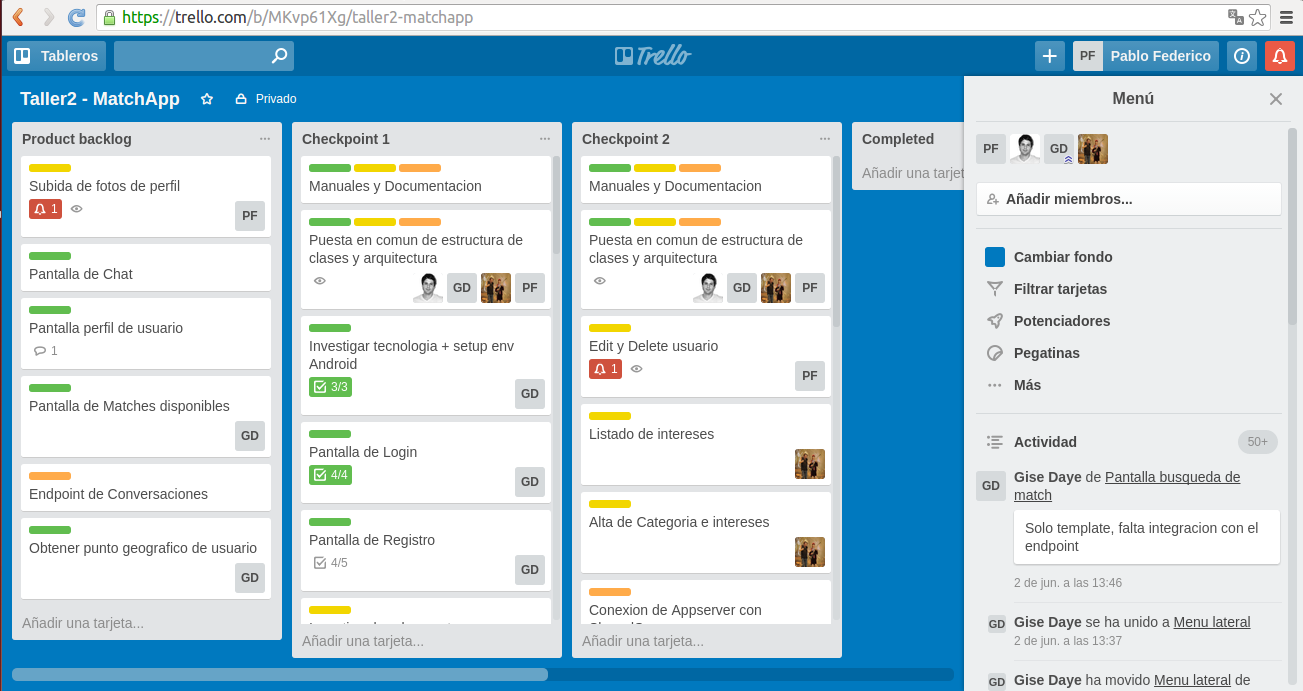
\includegraphics{trello.png}

\href{https://trello.com/b/MKvp61Xg/taller2-matchapp}{https://trello.com/b/MKvp61Xg/taller2-matchapp}
\begin{itemize}
\item {} \begin{description}
\item[{Repositorios taggeados en cada checkpoint}] \leavevmode\begin{itemize}
\item {} 
Shared Server: \href{https://github.com/PabloFederico/SharedServer}{https://github.com/PabloFederico/SharedServer}

\item {} 
App Server: \href{https://github.com/nicolas-vazquez/tp75521c}{https://github.com/nicolas-vazquez/tp75521c}

\item {} 
Cliente y Documentación: \href{https://github.com/gisedaye/taller2android}{https://github.com/gisedaye/taller2android}

\end{itemize}

\end{description}

\end{itemize}


\section{Entregas}
\label{manuals:entregas}

\subsection{Checkpoint 1}
\label{manuals:checkpoint-1}

\subsubsection{Changelog}
\label{manuals:changelog}\begin{itemize}
\item {} \begin{description}
\item[{Shared Server}] \leavevmode\begin{itemize}
\item {} 
Setup de la aplicación Heroku

\item {} 
Conexión con base de datos Postgres SQL

\item {} 
Webapp en Node.js con Listado, Alta, Baja y Modificación de perfiles de usuarios

\end{itemize}

\end{description}

\item {} \begin{description}
\item[{Application Server}] \leavevmode\begin{itemize}
\item {} 
CMake

\item {} 
Conexión con mongoose-cpp a RocksDB

\item {} 
Endpoints signup/login/like/dislike

\item {} 
Logs

\item {} 
Retornar Access Token en Login

\end{itemize}

\end{description}

\item {} \begin{description}
\item[{Cliente}] \leavevmode\begin{itemize}
\item {} 
Pantalla de Login

\item {} 
Pantalla de Registro

\item {} 
Integración con Appserver mediante Volley

\end{itemize}

\end{description}

\item {} 
Documentación

\end{itemize}


\subsubsection{División de tareas}
\label{manuals:division-de-tareas}\begin{itemize}
\item {} 
Cliente: Gisela

\item {} 
AppServer: Federico y Nicolás

\item {} 
SharedServer: Pablo

\end{itemize}

Trello Board para ver tareas y responsables:
\href{https://trello.com/b/MKvp61Xg/taller2-matchapp}{https://trello.com/b/MKvp61Xg/taller2-matchapp}


\subsubsection{Links útiles}
\label{manuals:links-utiles}

\paragraph{Repositorios}
\label{manuals:repositorios}\begin{itemize}
\item {} 
SharedServer: \href{https://github.com/PabloFederico/SharedServer}{https://github.com/PabloFederico/SharedServer}

\item {} 
ApplicationSever: \href{https://github.com/nicolas-vazquez/tp75521c}{https://github.com/nicolas-vazquez/tp75521c}

\item {} 
Cliente: \href{https://github.com/gisedaye/taller2android/}{https://github.com/gisedaye/taller2android/}

\end{itemize}


\paragraph{Aplicación web}
\label{manuals:aplicacion-web}
\href{https://tallerdeprogramacionii-1c2016.herokuapp.com/}{https://tallerdeprogramacionii-1c2016.herokuapp.com/}


\subsection{Checkpoint 2}
\label{manuals:checkpoint-2}

\subsubsection{Changelog}
\label{manuals:id1}\begin{itemize}
\item {} \begin{description}
\item[{Shared Server}] \leavevmode\begin{itemize}
\item {} 
Webapp en Node.js con Listado, Alta, Baja y Modificación de perfiles de usuarios

\item {} 
Listado de intereses

\item {} 
Alta de intereses

\item {} 
Docker en Shared server

\end{itemize}

\end{description}

\item {} \begin{description}
\item[{Application Server}] \leavevmode\begin{itemize}
\item {} 
Conexión de App Server con Shared Server

\item {} 
Lógica de Matches

\item {} 
Unit tests

\item {} 
CI-Travis

\item {} 
Docker en App Server

\end{itemize}

\end{description}

\item {} \begin{description}
\item[{Cliente}] \leavevmode\begin{itemize}
\item {} 
Pantalla de candidatos

\item {} 
Funcionalidad de like/dislike

\item {} 
Menú lateral

\end{itemize}

\end{description}

\item {} 
Documentación en Sphinx

\end{itemize}


\subsubsection{División de tareas}
\label{manuals:id2}\begin{itemize}
\item {} 
Cliente: Gisela

\item {} 
AppServer: Federico y Nicolás

\item {} 
SharedServer: Pablo y Nicolás

\end{itemize}

Trello Board para ver tareas y responsables:
\href{https://trello.com/b/MKvp61Xg/taller2-matchapp}{https://trello.com/b/MKvp61Xg/taller2-matchapp}


\subsubsection{Links útiles}
\label{manuals:id3}

\paragraph{Repositorios}
\label{manuals:id4}\begin{itemize}
\item {} 
SharedServer: \href{https://github.com/PabloFederico/SharedServer}{https://github.com/PabloFederico/SharedServer}

\item {} 
ApplicationSever: \href{https://github.com/nicolas-vazquez/tp75521c}{https://github.com/nicolas-vazquez/tp75521c}

\item {} 
Cliente: \href{https://github.com/gisedaye/taller2android/}{https://github.com/gisedaye/taller2android/}

\end{itemize}


\paragraph{Aplicación web}
\label{manuals:id5}
\href{https://tallerdeprogramacionii-1c2016.herokuapp.com/}{https://tallerdeprogramacionii-1c2016.herokuapp.com/}


\subsection{Checkpoint 3}
\label{manuals:checkpoint-3}

\subsubsection{Changelog}
\label{manuals:id6}\begin{itemize}
\item {} \begin{description}
\item[{Shared Server}] \leavevmode\begin{itemize}
\item {} 
Webapp en Node.js

\item {} 
Layout responsive con Materialize

\item {} 
Alta de intereses en usuarios

\item {} 
Alta de imagen en usuario

\item {} 
Localización de usuario

\item {} 
Endpoints login/interests/candidates/profile

\end{itemize}

\end{description}

\item {} \begin{description}
\item[{Application Server}] \leavevmode\begin{itemize}
\item {} 
Endpoints matches/candidates/messages/message/

\item {} 
Unit tests

\item {} 
Functional tests

\item {} 
Medir code coverage de unit tests

\end{itemize}

\end{description}

\item {} \begin{description}
\item[{Cliente}] \leavevmode\begin{itemize}
\item {} 
Pantalla de candidatos

\item {} 
Funcionalidad de like/dislike

\item {} 
Menú lateral

\item {} 
Pantalla de matches

\item {} 
Chat

\item {} 
Profile

\end{itemize}

\end{description}

\item {} 
Documentación en Sphinx

\end{itemize}


\subsubsection{División de tareas}
\label{manuals:id7}\begin{itemize}
\item {} 
Cliente: Federico

\item {} 
AppServer:  Federico y Nicolás

\item {} 
SharedServer: Federico y Nicolás

\item {} 
Shared server redesign: Gisela

\item {} 
Tests unitarios y funcionales: Gisela

\item {} 
Documentación: Gisela y Pablo

\end{itemize}

Trello Board para ver tareas y responsables:
\href{https://trello.com/b/MKvp61Xg/taller2-matchapp}{https://trello.com/b/MKvp61Xg/taller2-matchapp}


\section{Links útiles}
\label{manuals:id8}\begin{itemize}
\item {} 
SharedServer: \href{https://github.com/PabloFederico/SharedServer}{https://github.com/PabloFederico/SharedServer}

\item {} 
ApplicationSever: \href{https://github.com/nicolas-vazquez/tp75521c}{https://github.com/nicolas-vazquez/tp75521c}

\item {} 
Cliente: \href{https://github.com/gisedaye/taller2android/}{https://github.com/gisedaye/taller2android/}

\end{itemize}

\href{https://tallerdeprogramacionii-1c2016.herokuapp.com/}{https://tallerdeprogramacionii-1c2016.herokuapp.com/}


\section{Hipótesis y Supuestos}
\label{manuals:hipotesis-y-supuestos}\begin{itemize}
\item {} 
El usuario tendrá conocimientos en la utilización de un Sistema Operativo y contará con un dispositivo móvil con una adecuada conexión para el correcto funcionamiento del aplicativo.

\item {} 
La documentación del sistema (manuales de usuario, proyecto, administración y programador) será escrita en Español.

\end{itemize}


\section{Lecciones Aprendidas}
\label{manuals:lecciones-aprendidas}\begin{itemize}
\item {} 
Decidimos separar las tareas sin tener en cuenta las tecnologías que manejaba cada integrante y eso nos hizo atrasarnos en los primeros checkpoints.

\item {} 
Importancia de llevar un backlog de tareas, a fín de organizar el proyecto y el trabajo en grupo.

\item {} 
Estimación de tareas y control de tickets.

\item {} 
Integración en un solo aplicativo de varias tecnologías.

\item {} 
Importancia de utilizar Docker para el despliegue de la aplicación de manera de proveer una capa de abstracción.

\item {} 
Utilizar el tiempo para plantear una solución de calidad tanto en arquitectura como en diseño al comienzo del proyecto es de vital importancia para lograr el éxito del mismo y minimizar los riesgos futuros.

\end{itemize}


\chapter{Indices y tablas}
\label{index:indices-y-tablas}\begin{itemize}
\item {} 
\emph{genindex}

\item {} 
\emph{modindex}

\item {} 
\emph{search}

\end{itemize}



\renewcommand{\indexname}{Index}
\printindex
\end{document}
